\documentclass{article}
\usepackage[margin=1in]{geometry}
\usepackage{problemset}
\showsolntrue

% Custom commands
\newcommand{\R}{\mathbb{R}}
\newcommand{\X}{\mathcal{X}}
\newcommand{\Y}{\mathcal{Y}}

\begin{document}

\pstitle{%
    CSE 151A%
}{
    Homework 7%
}[due Thursday, May 22 at 11:59PM]

\textbf{Instructions:}
\begin{itemize}
    \item You may discuss problems with your study group, but ultimately all your work (mathematical problems, code, experimental details) must be individual.
    \item Your solutions must be \texttt{typed up} and uploaded to Gradescope by 11.59PM on Thursday May X. No late homeworks will be accepted under any circumstances, so you are encouraged to upload early.
    \item A subset of the problems will be graded.
\end{itemize}

\begin{probset}
\begin{prob}
    Draw the decision boundary in $\R^2$ that corresponds to the prediction rule sign$(2x_1 - x_2 - 6)$. Make sure to clearly indicate where this boundary intersects the axes. Show which side of the boundary is classified as positive and which side as negative.

    \begin{soln}
        The shaded region is the set of points that are classified as positive, and the unshaded region is the set of points that are classified as negative.
        \begin{center}
            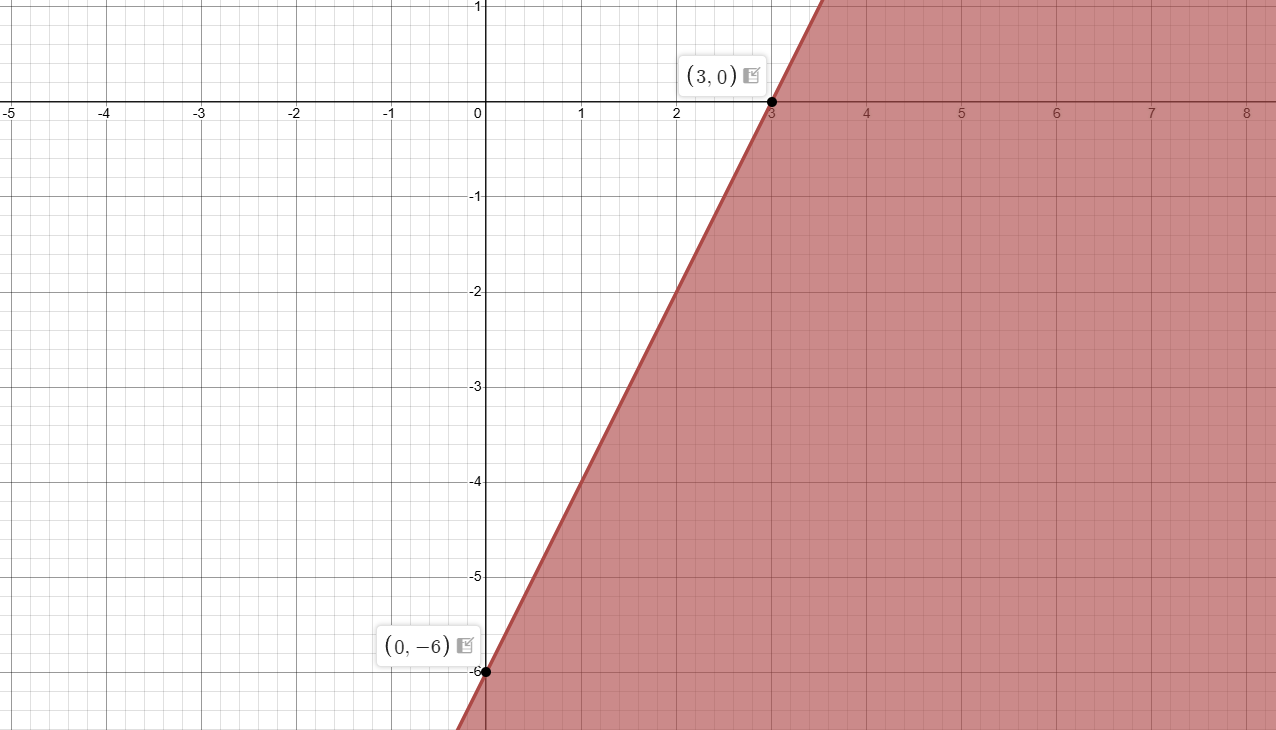
\includegraphics[width=0.4\textwidth]{Images/1.png}
        \end{center}
    \end{soln}
\end{prob}

\newpage

\begin{prob}
    A particular labeled data of n points is randomly permuted and then the Perceptron algorithm is run on it, repeatedly cycling through the points until convergence. It converges after making $k$ updates. For each of the following statements, say whether it is \textbf{definitely true} or \textbf{possibly false}, and give a brief reason.

    \begin{subprobset}
    \begin{subprob}
        The data is linearly separable.

        \begin{soln}
            This is definitely true because the Perceptron algorithm converges if and only if the data is linearly separable.
        \end{soln}
    \end{subprob}
    \begin{subprob}
        If the process were repeated with a different random permutation, it would again converge.

        \begin{soln}
            This is definitely true because convergence is guaranteed regardless of permutation since the data is linearly separable.
        \end{soln}
    \end{subprob}

    \begin{subprob}
        If the process were repeated with a different random permutation, it would again converge after making $k$ updates.
        
        \begin{soln}
            This is possibly false because the number of updates can vary with different permutations due to the order in which mistakes are corrected.
        \end{soln}
    \end{subprob}

    \begin{subprob}
        $k$ is at most $n$.
        
        \begin{soln}
            This is possibly false because the number of updates can exceed $n$ as the algorithm may cycle through the data multiple times.
        \end{soln}
    \end{subprob}
    \end{subprobset}
\end{prob}

\begin{prob}
    The Perceptron algorithm is run on a data set, and converges after performing $p + q$ updates. Of these updates, $p$ are on data points whose label is $-1$ and $q$ are on data points whose label is $+1$. What is the final value of the parameter $b$?

    \begin{soln}
        \[ b = \sum_{i=1}^{q} 1 + \sum_{i=1}^{p} -1 = q - p \]
    \end{soln}
\end{prob}

\newpage

\begin{prob}
    An SVM classifier is learned for a data set in $\R^2$. It is given by $w = \begin{bmatrix} 3 \\ 4 \end{bmatrix}$ and $b = -12$.

    \begin{subprobset}
    \begin{subprob}
        Draw the decision boundary, making sure to clearly indicate where it intersects the axes.

        \begin{soln}
            \begin{center}
                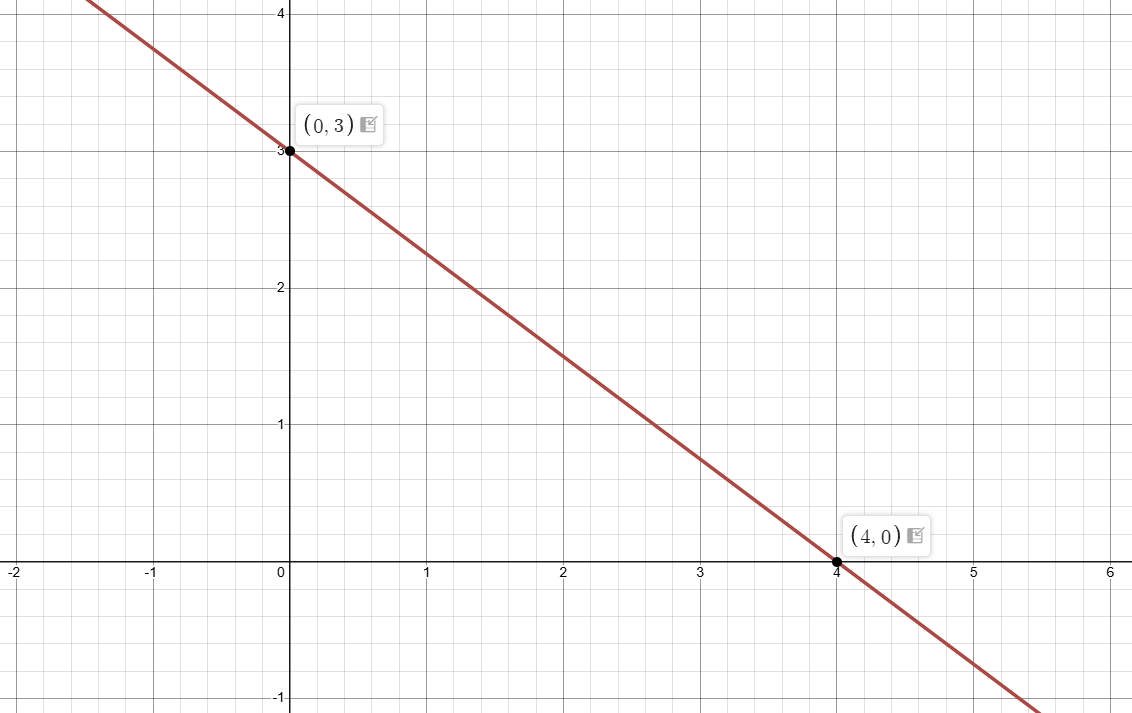
\includegraphics[width=0.4\textwidth]{Images/4a.png}
            \end{center}
        \end{soln}
    \end{subprob}

    \begin{subprob}
        Draw the left-hand and right-hand boundaries, also clearly marking where they intersect the axes.

        \begin{soln}
            \begin{center}
                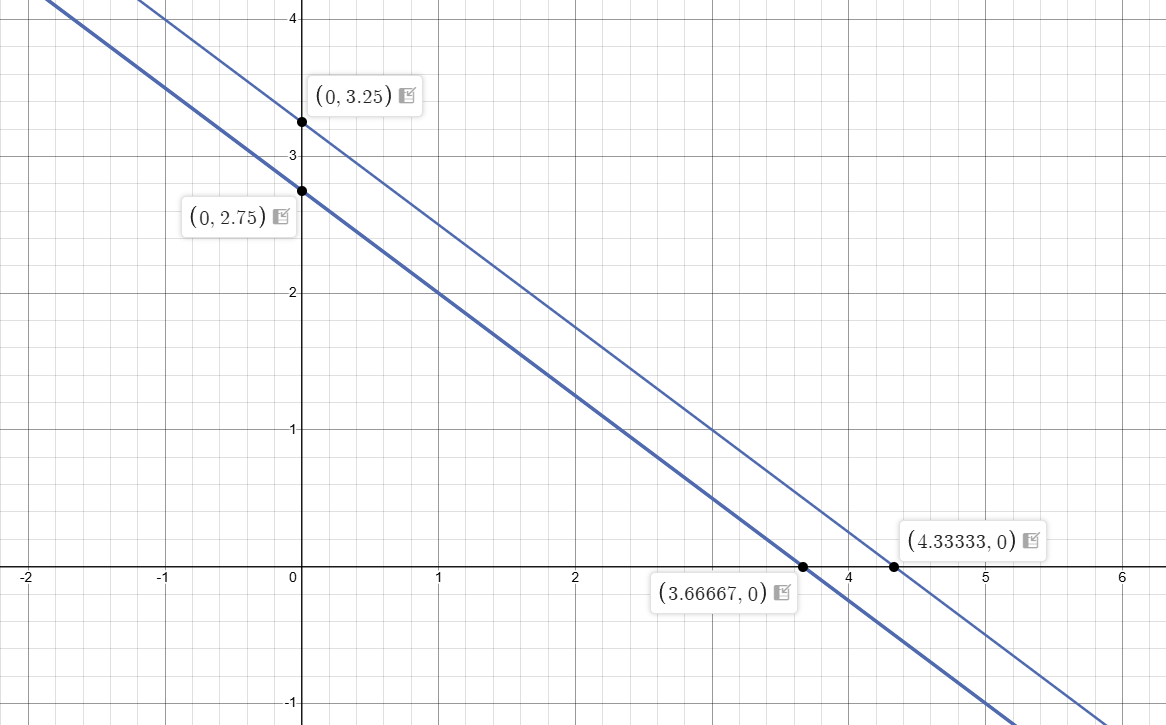
\includegraphics[width=0.4\textwidth]{Images/4b.png}
            \end{center}
        \end{soln}
    \end{subprob}

    \begin{subprob}
        What is the margin of this classifier?

        \begin{soln}
            The margin is the distance between the two boundaries, which is $\frac{2}{\|w\|} = \frac{2}{\sqrt{3^2 + 4^2}} = \frac{2}{5}$.
        \end{soln}
    \end{subprob}

    \begin{subprob}
        How would the point $\begin{bmatrix} 2 \\ 2 \end{bmatrix}$ be classified?

        \begin{soln}
            The point $\begin{bmatrix} 2 \\ 2 \end{bmatrix}$ is classified as positive because $w \cdot x + b = 3(2) + 4(2) - 12 = 2 > 0$.
        \end{soln}
    \end{subprob}
    \end{subprobset}
\end{prob}

\newpage

\begin{prob}
    The picture below shows the decision boundary obtained upon running soft-margin SVM on a small data set of blue squares and red circles.

    \begin{center}
        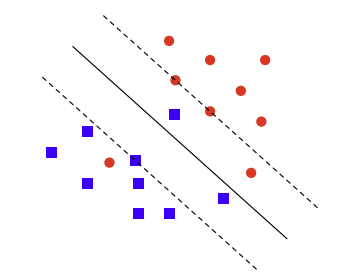
\includegraphics[width=0.4\textwidth]{Images/5.png}
    \end{center}

    \begin{subprobset}
    \begin{subprob}
        Copy this figure and mark the support vectors. For each, indicate the approximate value of the corresponding slack variable.

        \begin{soln}
            \begin{center}
                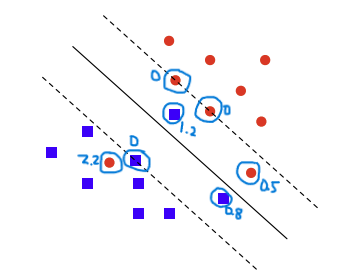
\includegraphics[width=0.4\textwidth]{Images/5a.png}
            \end{center}
        \end{soln}
    \end{subprob}

    \begin{subprob}
        Suppose the factor $C$ in the soft-margin SVM optimization problem were increased. Would you expect the margin to increase or decrease?

        \begin{soln}
            Increasing $C$ places a higher penalty on slack variables (misclassifications or margin violations). This forces the SVM to reduce violations by fitting the data more strictly, which usually results in a smaller margin to better separate the points.
        \end{soln}
    \end{subprob}
    \end{subprobset}
\end{prob}

\newpage

\begin{prob}
    (This problem is based on material from discussion section.) The dual form of the Perceptron algorithm is used to learn a binary classifier, based on $n$ training points. It converges after $k$ updates, and returns a vector $\alpha$ and a number $b$. For each of the following statements, indicate whether it is necessarily true or possibly false, and give a brief justification.

    \begin{subprobset}
    \begin{subprob}
        Each $\alpha_i$ is either 0 or 1.

        \begin{soln}
            This is possibly false because each $\alpha_i$ could be updated multiple times, so it is possible for it to be greater than 1.
        \end{soln}
    \end{subprob}

    \begin{subprob}
        $\sum_{i=1}^n \alpha_i = k$.

        \begin{soln}
            This is definitely true because the sum of the $\alpha_i$ is equal to the number of updates $k$.
        \end{soln}
    \end{subprob}

    \begin{subprob}
        $\alpha$ has at most $k$ nonzero coordinates.

        \begin{soln}
            This is definitely true because there were $k$ updates, so there are at most $k$ coordinates that were updated and are non-zero.
        \end{soln}
    \end{subprob}

    \begin{subprob}
        The training data must be linearly separable.

        \begin{soln}
            This is possibly false because the dual form of the Perceptron algorithm can converge even if the data is not linearly separable.
        \end{soln}
    \end{subprob}
    \end{subprobset}
\end{prob}

\newpage

\begin{progprob}[\textit{Binary Perceptron}]
    In this problem, you will code up the (binary) Perceptron algorithm and use it to classify the Iris data set.

    \begin{subprobset}
    \begin{subprob}
        Write code for two functions:

        \begin{itemize}
            \item The first function takes as input parameters $w, b$ of a linear classifier as well as a data point $x$, and returns the label for that point: sign$(w \cdot x + b)$. The label is either $+1$ or $-1$.
            \item The second function takes as input an array of data points and an array of labels (where each label is $+1$ or $-1$), and runs the Perceptron algorithm to learn a linear classifier $w, b$. The algorithm should begin by randomly permuting the data points.
        \end{itemize}

        In your writeup, give the code for these two functions.

        \begin{verbatim}
def classify(x, w, b):
    return np.sign(np.dot(x, w) + b)

def perceptron(X, Y, epochs=100):
    perm = np.random.permutation(len(X))
    X = X[perm]
    Y = Y[perm]

    w = np.zeros(X.shape[1])
    b = 0
    updates_per_epoch = []

    for _ in range(epochs):
        updates = 0
        for x, y in zip(X, Y):
            if classify(x, w, b) != y:
                w += y * x
                b += y
                updates += 1
        updates_per_epoch.append(updates)
        if updates == 0:
            break

    return w, b, updates_per_epoch
        \end{verbatim}
    \end{subprob}

    \begin{subprob}
        Load in the Iris data set. You can do this by simply invoking:
        \begin{verbatim}
from sklearn import datasets
iris = datasets.load_iris()
X = iris.data
Y = iris.target
        \end{verbatim}

        The data has four features and three labels. Restrict it to features 1 and 3 (the second and fourth columns, sepal width and petal width) and to labels 0,1. Recode label 0 as -1, since this is what the Perceptron algorithm is expecting.

        \begin{verbatim}
X = X[Y != 2]
X = X[:, [1, 3]]
Y = Y[Y != 2]
Y[Y == 0] = -1
        \end{verbatim}
    \end{subprob}

    \newpage

    \begin{subprob}
        Now run the Perceptron algorithm on the data. In your writeup, show a plot with the data points (where the two labels have different colors) and the resulting decision boundary.

        \begin{soln}
            \begin{center}
                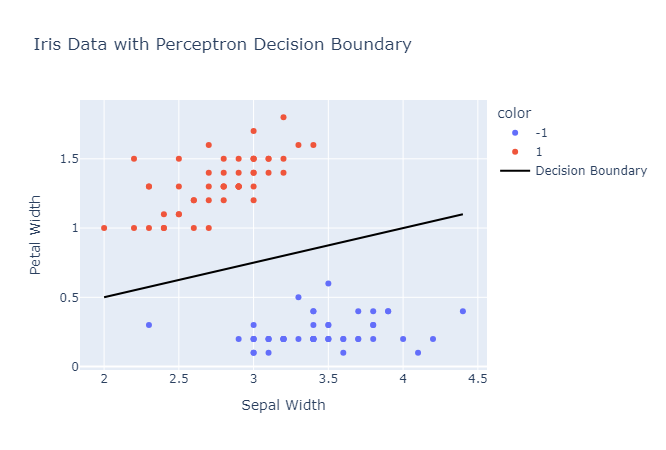
\includegraphics[width=0.6\textwidth]{Images/7c.png}
            \end{center}
        \end{soln}
    \end{subprob}

    \begin{subprob}
        Now modify your code from part (a) to count the \textit{number of updates} made by the Perceptron algorithm while it is learning. Run the algorithm 20 times and keep track of the number of updates needed each time. In your writeup, include a histogram of these values.

        \begin{soln}
            \begin{center}
                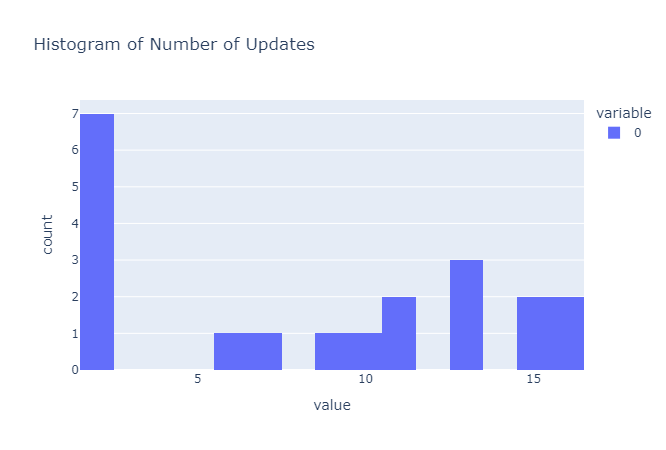
\includegraphics[width=0.6\textwidth]{Images/7d.png}
            \end{center}
        \end{soln}
    \end{subprob}
    \end{subprobset}
\end{progprob}

\newpage

\begin{progprob}[\textit{Support vector machine}]
    As you did with the Perceptron, use the Iris data set, but this time use features 0 and 2, and labels 1,2.

    \begin{subprobset}
    \begin{subprob}
        Is this data linearly separable?

        \begin{soln}
            No, the data is not linearly separable because the convex hulls of the two classes overlap.
        \end{soln}
    \end{subprob}

    \begin{subprob}
        Use \texttt{sklearn.svm.SVC} to fit a support vector machine classifier to the data. You will need to invoke the option \texttt{kernel='linear'}. Try at least 10 different values of the slack parameter $C$. In your writeup, include a table that shows these values of $C$ and for each of them gives the training error and the number of support vectors.

        \begin{soln}
            \begin{center}
                \begin{tabular}{lrr}
                    \toprule
                    $C$ & Training Error & Support Vectors \\
                    \midrule
                    $0.0001$ & $0.17$ & $100$ \\
                    $0.001$ & $0.17$ & $100$ \\
                    $0.01$ & $0.16$ & $92$ \\
                    $0.1$ & $0.07$ & $56$ \\
                    $1$ & $0.07$ & $32$ \\
                    $10$ & $0.05$ & $18$ \\
                    $100$ & $0.05$ & $14$ \\
                    $1000$ & $0.05$ & $14$ \\
                    $10000$ & $0.05$ & $14$ \\
                    $100000$ & $0.06$ & $14$ \\
                \end{tabular}
            \end{center}
        \end{soln}
    \end{subprob}

    \begin{subprob}
        Which value of $C$ do you think is best? For this value, include a plot of the data points and the linear decision boundary.

        \begin{soln}
            I would choose $C = 10$ because it's the lowest $C$ with the lowest training error. Choosing a higher $C$ would increase the chance of overfitting.

            \begin{center}
                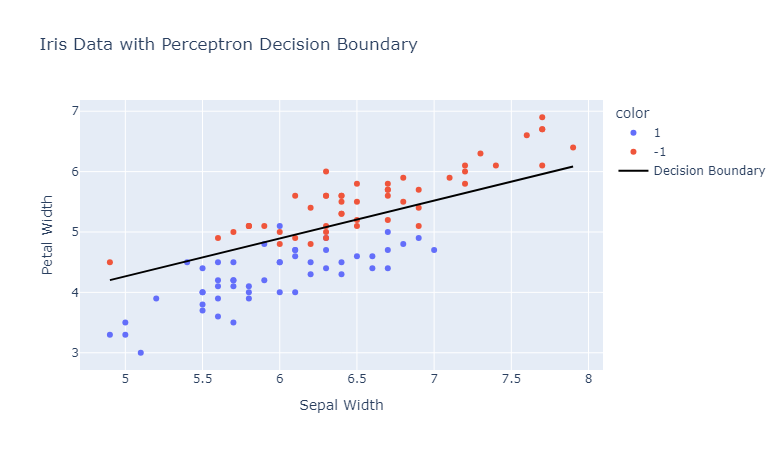
\includegraphics[width=0.6\textwidth]{Images/8c.png}
            \end{center}
        \end{soln}
    \end{subprob}
    \end{subprobset}
\end{progprob}
\end{probset}
\end{document}